\documentclass[11pt,a4paper]{report}
\usepackage[textwidth=37em,vmargin=30mm]{geometry}
\usepackage{calc,xunicode,amsmath,amssymb,paralist,enumitem,tabu,booktabs,datetime2,xeCJK,xeCJKfntef,listings}
\usepackage{tocloft,fancyhdr,tcolorbox,xcolor,graphicx,eso-pic,xltxtra,xelatexemoji}

\newcommand{\envyear}[0]{2024}
\newcommand{\envdatestr}[0]{2024-11-06}
\newcommand{\envfinaldir}[0]{webdb/2024/20241106/final}

\usepackage[hidelinks]{hyperref}
\hypersetup{
    colorlinks=false,
    pdfpagemode=FullScreen,
    pdftitle={Web Digest - \envdatestr}
}

\setlength{\cftbeforechapskip}{10pt}
\renewcommand{\cftchapfont}{\rmfamily\bfseries\large\raggedright}
\setlength{\cftbeforesecskip}{2pt}
\renewcommand{\cftsecfont}{\sffamily\small\raggedright}

\setdefaultleftmargin{2em}{2em}{1em}{1em}{1em}{1em}

\usepackage{xeCJK,xeCJKfntef}
\xeCJKsetup{PunctStyle=plain,RubberPunctSkip=false,CJKglue=\strut\hskip 0pt plus 0.1em minus 0.05em,CJKecglue=\strut\hskip 0.22em plus 0.2em}
\XeTeXlinebreaklocale "zh"
\XeTeXlinebreakskip = 0pt


\setmainfont{Brygada 1918}
\setromanfont{Brygada 1918}
\setsansfont{IBM Plex Sans}
\setmonofont{JetBrains Mono NL}
\setCJKmainfont{Noto Serif CJK SC}
\setCJKromanfont{Noto Serif CJK SC}
\setCJKsansfont{Noto Sans CJK SC}
\setCJKmonofont{Noto Sans CJK SC}

\setlength{\parindent}{0pt}
\setlength{\parskip}{8pt}
\linespread{1.15}

\lstset{
	basicstyle=\ttfamily\footnotesize,
	numbersep=5pt,
	backgroundcolor=\color{black!5},
	showspaces=false,
	showstringspaces=false,
	showtabs=false,
	tabsize=2,
	captionpos=b,
	breaklines=true,
	breakatwhitespace=true,
	breakautoindent=true,
	linewidth=\textwidth
}






\newcommand{\coverpic}[2]{
    % argv: itemurl, authorname
    Cover photo by #2~~(\href{#1}{#1})
}
\newcommand{\makeheader}[0]{
    \begin{titlepage}
        % \newgeometry{hmargin=15mm,tmargin=21mm,bmargin=12mm}
        \begin{center}
            
            \rmfamily\scshape
            \fontspec{BaskervilleF}
            \fontspec{Old Standard}
            \fontsize{59pt}{70pt}\selectfont
            WEB\hfill DIGEST
            
            \vfill
            % \vskip 30pt
            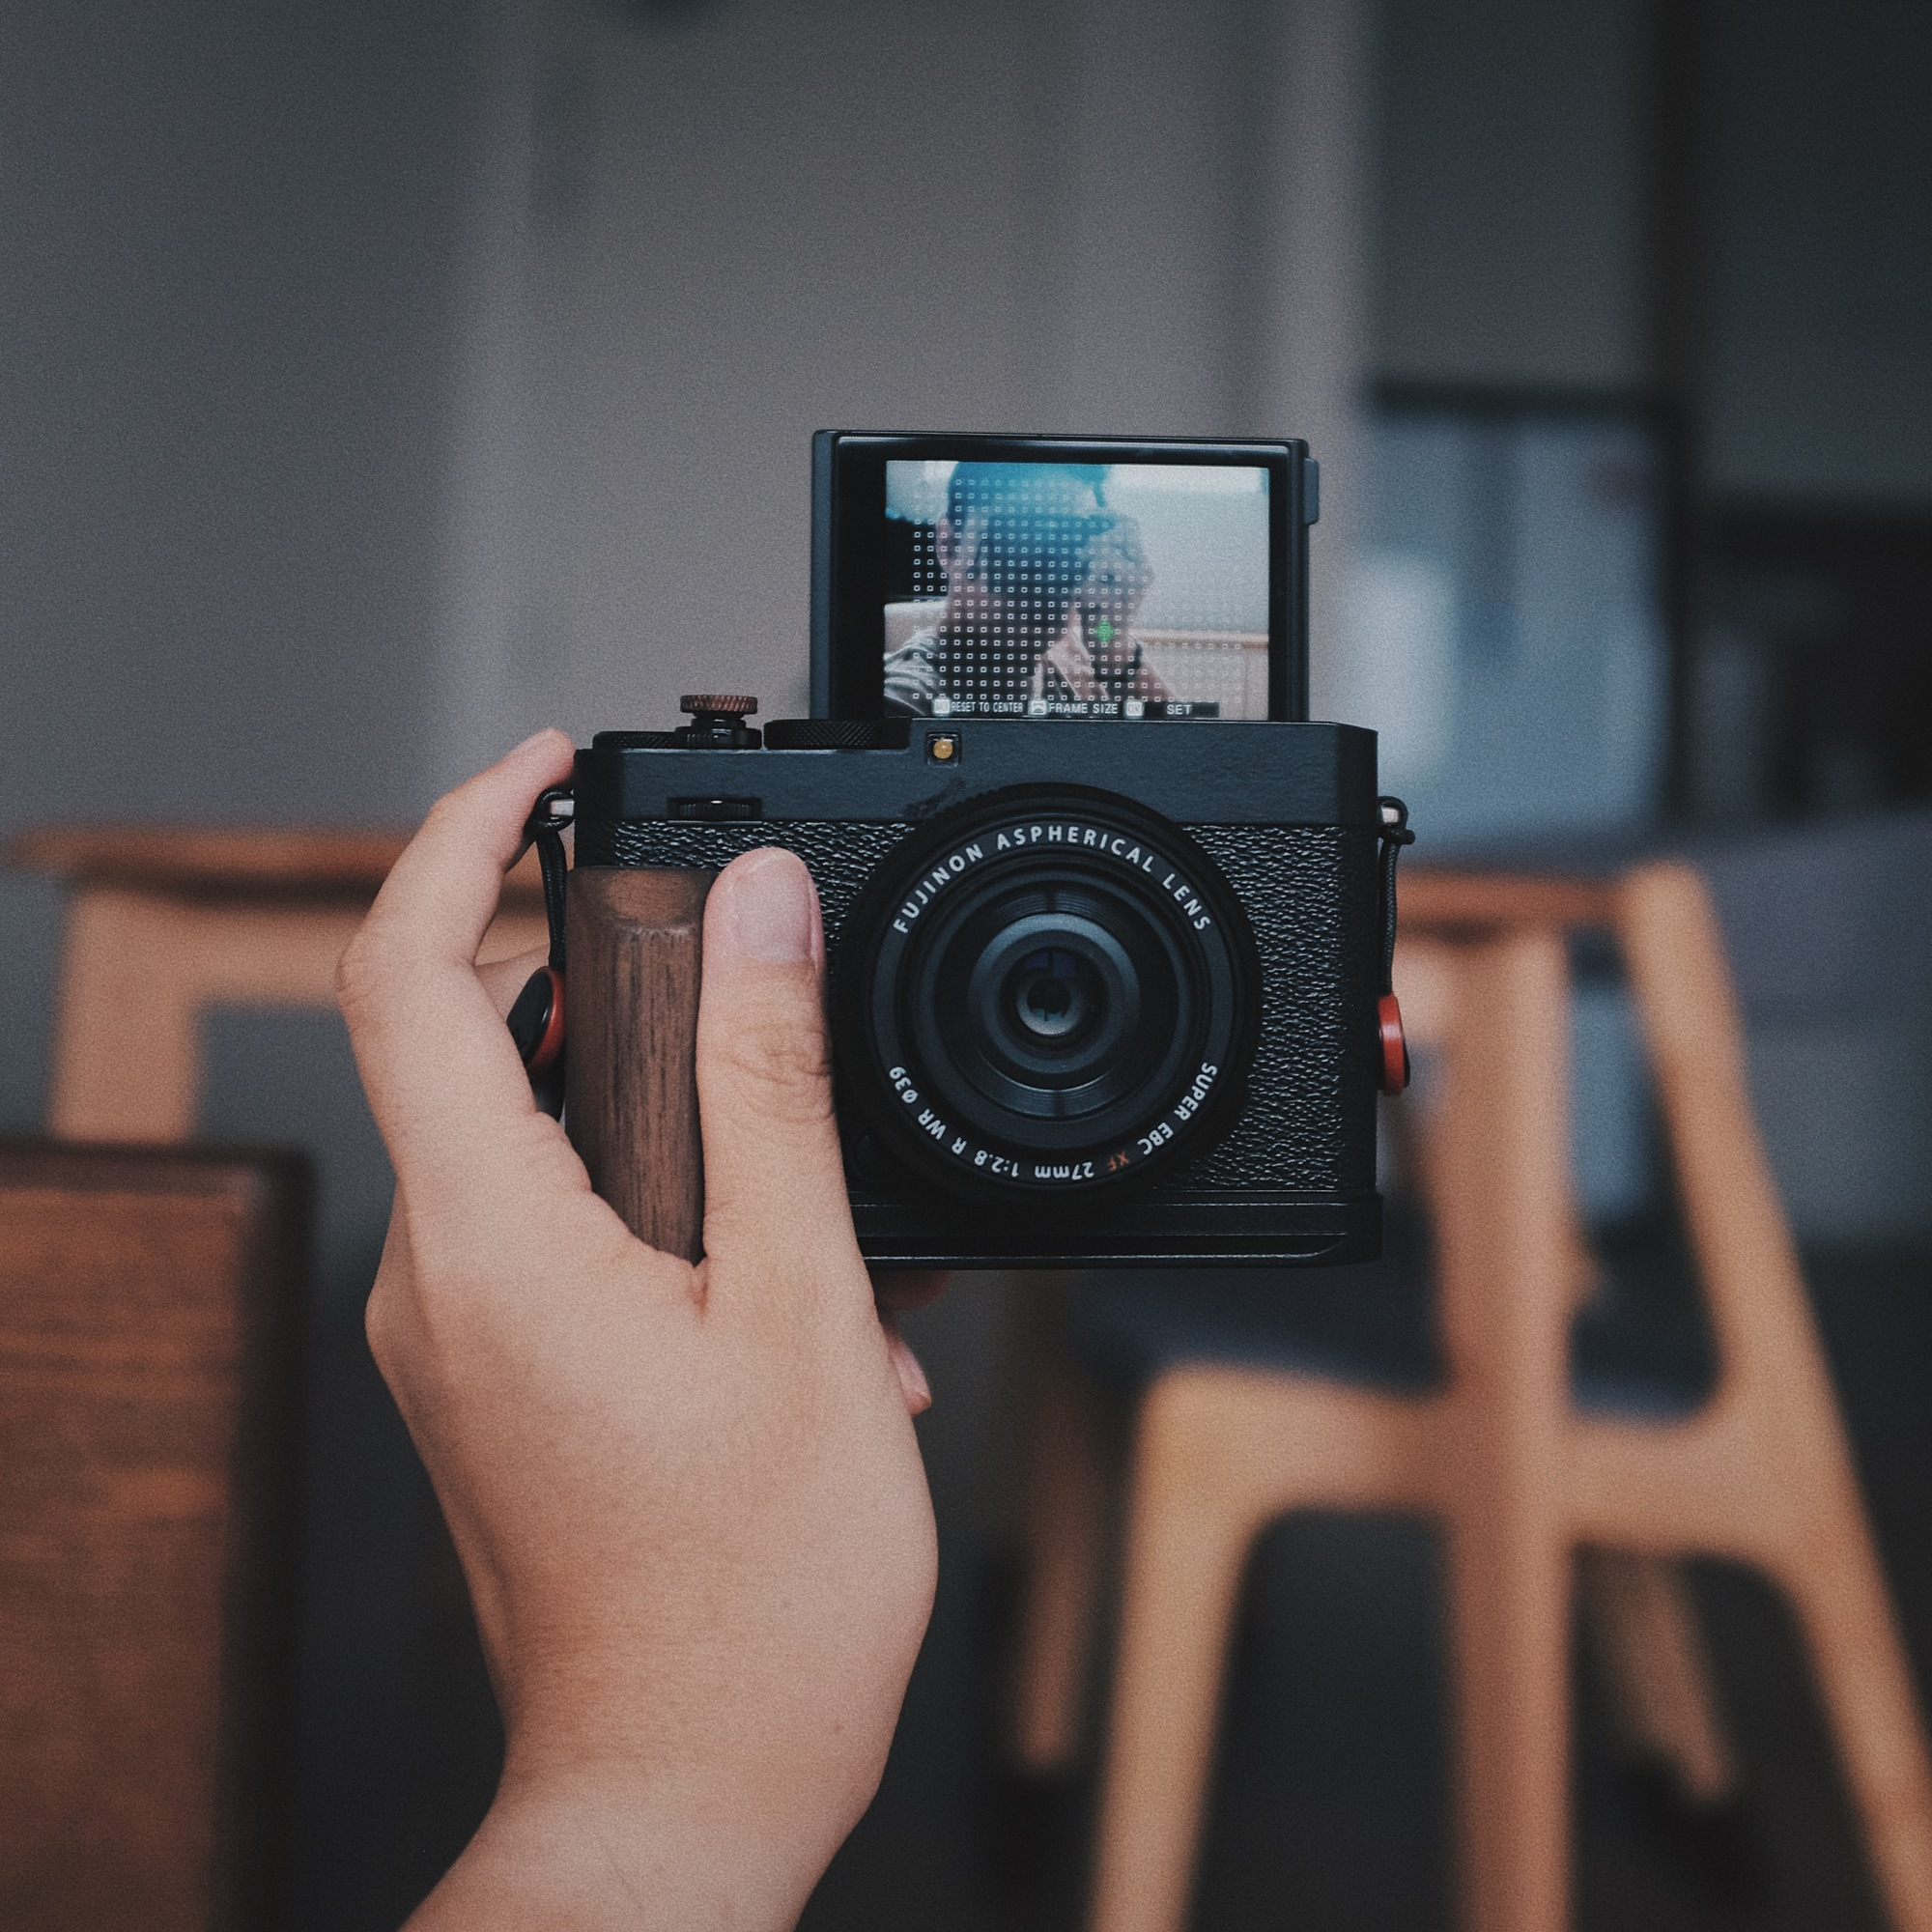
\includegraphics[width=\linewidth]{\envfinaldir/coverpic-prod.jpg}\par
            % \vskip 30pt
            \vfill

            \normalsize\rmfamily\scshape
            \copyright{} The Web Digest Project \hfill\large \envdatestr
        \end{center}
    \end{titlepage}
    % \restoregeometry
}
\newcommand{\simplehref}[1]{%
    \textcolor{blue!80!green}{\href{#1}{#1}}%
}
\renewcommand{\contentsname}{\center\Huge\sffamily\bfseries Contents\par\vskip 20pt}
\newcounter{ipartcounter}
\setcounter{ipartcounter}{0}
\newcommand{\ipart}[1]{
    % \vskip 20pt
    \clearpage
    \stepcounter{ipartcounter}
    \phantomsection
    \addcontentsline{toc}{chapter}{#1}
    % \begin{center}
    %     \Huge
    %     \sffamily\bfseries
    %     #1
    % \end{center}
    % \vskip 20pt plus 7pt
}
\newcounter{ichaptercounter}
\setcounter{ichaptercounter}{0}
\newcommand{\ichapter}[1]{
    % \vskip 20pt
    \clearpage
    \stepcounter{ichaptercounter}
    \phantomsection
    \addcontentsline{toc}{section}{\numberline{\arabic{ichaptercounter}}#1}
    \begin{center}
        \Huge
        \sffamily\bfseries
        #1
    \end{center}
    \vskip 20pt plus 7pt
}
\newcommand{\entrytitlefont}[1]{\subsection*{\raggedright\Large\sffamily\bfseries#1}}
\newcommand{\entryitemGeneric}[2]{
    % argv: title, url
    \parbox{\linewidth}{
        \entrytitlefont{#1}\par\vskip 5pt
        \footnotesize\ttfamily\mdseries
        \simplehref{#2}
    }\vskip 11pt plus 11pt minus 1pt
}
\newcommand{\entryitemGithub}[3]{
    % argv: title, url, desc
    \parbox{\linewidth}{
        \entrytitlefont{#1}\par\vskip 5pt
        \footnotesize\ttfamily\mdseries
        \simplehref{#2}\par\vskip 5pt
        \small\rmfamily\mdseries#3
    }\vskip 11pt plus 11pt minus 1pt
}
\newcommand{\entryitemAp}[3]{
    % argv: title, url, desc
    \parbox{\linewidth}{
        \entrytitlefont{#1}\par\vskip 5pt
        \footnotesize\ttfamily\mdseries
        \simplehref{#2}\par\vskip 5pt
        \small\rmfamily\mdseries#3
    }\vskip 11pt plus 11pt minus 1pt
}
\newcommand{\entryitemHackernews}[3]{
    % argv: title, hnurl, rawurl
    % \parbox{\linewidth}{
    %     \entrytitlefont{#1}\par\vskip 5pt
    %     \footnotesize\ttfamily\mdseries
    %     \simplehref{#3}\par
    %     \textcolor{black!50}{\href{#2}{#2}}
    % }\vskip 11pt plus 11pt minus 1pt
    \begin{minipage}{\linewidth}
            \entrytitlefont{#1}\par\vskip 5pt
            \footnotesize\ttfamily\mdseries
            \simplehref{#3}\par
            \textcolor{black!50}{\href{#2}{#2}}
    \end{minipage}\par\vskip 11pt plus 11pt minus 1pt
}







\begin{document}

\makeheader

\tableofcontents\clearpage




\ipart{Developers}
\ichapter{Hacker News}
\entryitemTwoLinks{Boeing ends crippling strike as workers accept latest offer}{https://news.ycombinator.com/item?id=42052263}{https://www.bloomberg.com/news/articles/2024-11-05/boeing-ends-crippling-strike-after-workers-accept-latest-offer}

\entryitemTwoLinks{Hacking 700M Electronic Arts accounts}{https://news.ycombinator.com/item?id=42052143}{https://battleda.sh/blog/ea-account-takeover}

\entryitemTwoLinks{New documentary reveals that 21,000 laborers have died working Saudi Vision 2030}{https://news.ycombinator.com/item?id=42052105}{https://www.archpaper.com/2024/10/documentary-reveals-21000-workers-killed-saudi-vision-2030-neom/}

\entryitemTwoLinks{Why shouldn't you give money to homeless people?}{https://news.ycombinator.com/item?id=42051651}{https://spiralprogress.com/2024/11/04/why-shouldnt-you-give-money-to-homeless-people/}

\entryitemTwoLinks{Netflix Europe offices raided in tax fraud probe}{https://news.ycombinator.com/item?id=42051643}{https://www.bbc.co.uk/news/articles/cwy1vze09wwo}

\entryitemTwoLinks{Study reveals blood sugar control is a key factor in slowing brain aging}{https://news.ycombinator.com/item?id=42049418}{https://www.bgu.ac.il/en/news-and-articles/blood-sugar-control-is-key-factor-in-slowing-brain-aging/}

\entryitemTwoLinks{Programmer in Berlin: Culture}{https://news.ycombinator.com/item?id=42049180}{https://wickedchicken.github.io/post/programmer-in-berlin-culture/}

\entryitemTwoLinks{The average age of U.S. homebuyers jumps to 56}{https://news.ycombinator.com/item?id=42048640}{https://www.cnbc.com/2024/11/04/homebuyer-average-age-rises-to-56-amid-rising-homeownership-costs.html}

\entryitemTwoLinks{Nvidia and its partners built a system to bypass U.S. export restrictions}{https://news.ycombinator.com/item?id=42048065}{https://twitter.com/kakashiii111/status/1853433531260649532}

\entryitemTwoLinks{Meta Permits Its A.I. Models to Be Used for U.S. Military Purposes}{https://news.ycombinator.com/item?id=42048009}{https://www.nytimes.com/2024/11/04/technology/meta-ai-military.html}

\entryitemTwoLinks{Pagination widows, or, why I'm embarrassed about my eBook (2023)}{https://news.ycombinator.com/item?id=42047677}{https://clagnut.com/blog/2426}

\entryitemTwoLinks{USFS decision to halt prescribed burns in California is history repeating}{https://news.ycombinator.com/item?id=42046596}{https://cepr.net/us-forest-service-decision-to-halt-prescribed-burns-in-california-is-history-repeating/}

\entryitemTwoLinks{Albertsons kills rural grocers with land use restrictions}{https://news.ycombinator.com/item?id=42046196}{https://www.thebignewsletter.com/p/how-albertsons-kills-rural-grocers}

\entryitemTwoLinks{Diagram as Code}{https://news.ycombinator.com/item?id=42044771}{https://diagrams.mingrammer.com/}

\entryitemTwoLinks{Writing secure Go code}{https://news.ycombinator.com/item?id=42043939}{https://jarosz.dev/article/writing-secure-go-code/}

\entryitemTwoLinks{DB48X: High Performance Scientific Calculator, Reinvented}{https://news.ycombinator.com/item?id=42043747}{http://48calc.org/}

\entryitemTwoLinks{Manjaro Linux prepares to enable telemetry by default}{https://news.ycombinator.com/item?id=42043539}{https://forum.manjaro.org/t/testers-needed-manjaro-data-donor/170163}

\entryitemTwoLinks{What should a logo for NeXT look like? (1986)}{https://news.ycombinator.com/item?id=42042382}{https://www.paulrand.design/work/NeXT-Computers.html}

\entryitemTwoLinks{We're Leaving Kubernetes}{https://news.ycombinator.com/item?id=42041917}{https://www.gitpod.io/blog/we-are-leaving-kubernetes}

\entryitemTwoLinks{Facebook building subsea cable that will encompass the world}{https://news.ycombinator.com/item?id=42041581}{https://subseacables.blogspot.com/2024/10/breaking-story-facebook-building-subsea.html}\ichapter{Phoronix}
\entryitemGeneric{\hskip 0pt{}GIMP 3.0 RC1 Released For Testing}{https://www.phoronix.com/news/GIMP-3.0-RC1}

\entryitemGeneric{\hskip 0pt{}Power Determinism Mode Still Proves Beneficial For AMD EPYC 9005 Performance}{https://www.phoronix.com/review/amd-epyc-9005-determinism}

\entryitemGeneric{\hskip 0pt{}Open-Source PowerVR Driver Being Extended For The Imagination BXS-4-64 MC1 GPU}{https://www.phoronix.com/news/PVR-Imagination-BXS-4-64-MC1}

\entryitemGeneric{\hskip 0pt{}Linux 6.13 To Drop Fieldbus Just Five Years After Being Merged}{https://www.phoronix.com/news/Linux-6.13-Dropping-Fieldbus}

\entryitemGeneric{\hskip 0pt{}Linux 6.13 To Enhance Logic For Trusting Built-In Thunderbolt Controllers}{https://www.phoronix.com/news/Linux-6.13-Thunderbolt-Trust}

\entryitemGeneric{\hskip 0pt{}LXQt 2.1 Released With New Wayland Session Component}{https://www.phoronix.com/news/LXQt-2.1-Released}

\entryitemGeneric{\hskip 0pt{}Intel Panther Lake Display Support Squeezing Into Linux 6.13}{https://www.phoronix.com/news/Intel-Panther-Lake-Display-6.13}

\entryitemGeneric{\hskip 0pt{}Intel Releases x86-simd-sort 6.0 For Speedy AVX2/AVX-512 Sorting, PyTorch Now Using It}{https://www.phoronix.com/news/x86-simd-sort-6.0}

\entryitemGeneric{\hskip 0pt{}Linux Preps New AMD ERAPS Feature With EPYC Turin To Benefit Performance}{https://www.phoronix.com/news/AMD-ERAPS-Linux}\ichapter{Dribbble}
\entryitemGeneric{\hskip 0pt{}Lootbox}{https://dribbble.com/shots/24875582}

\entryitemGeneric{\hskip 0pt{}Internal Universe 🪐✨}{https://dribbble.com/shots/24870294}

\entryitemGeneric{\hskip 0pt{}Gulfstream x theory11 Playing Cards}{https://dribbble.com/shots/24869176}

\entryitemGeneric{\hskip 0pt{}Negative yet Positive Vol.7}{https://dribbble.com/shots/24868890}

\entryitemGeneric{\hskip 0pt{}Onton - Responsive Logo Design}{https://dribbble.com/shots/24866015}

\entryitemGeneric{\hskip 0pt{}Solufacil}{https://dribbble.com/shots/24869750}

\entryitemGeneric{\hskip 0pt{}Raw E}{https://dribbble.com/shots/24869489}

\entryitemGeneric{\hskip 0pt{}Ampersand 3D Logo}{https://dribbble.com/shots/24869500}

\entryitemGeneric{\hskip 0pt{}Rooster}{https://dribbble.com/shots/24854380}

\entryitemGeneric{\hskip 0pt{}cipher}{https://dribbble.com/shots/24855823}

\entryitemGeneric{\hskip 0pt{}"Amphiprion Ocellaris" - Daily art, NFT art}{https://dribbble.com/shots/24854577}

\entryitemGeneric{\hskip 0pt{}Bento Cards v.4 – E-Commerce}{https://dribbble.com/shots/24849627}

\entryitemGeneric{\hskip 0pt{}Neobanking Mobile App Interactions}{https://dribbble.com/shots/24848696}

\entryitemGeneric{\hskip 0pt{}FC Shakhtar Donetsk App. The Concept. Part 2}{https://dribbble.com/shots/24848383}

\entryitemGeneric{\hskip 0pt{}xflow Logo Design - X, Waves}{https://dribbble.com/shots/24847689}

\entryitemGeneric{\hskip 0pt{}The Future has landed ✈️}{https://dribbble.com/shots/24848230}

\entryitemGeneric{\hskip 0pt{}Converse Logo Redesign Concept}{https://dribbble.com/shots/24850036}

\entryitemGeneric{\hskip 0pt{}F Logo}{https://dribbble.com/shots/24850079}

\entryitemGeneric{\hskip 0pt{}ML Fashion 10/10}{https://dribbble.com/shots/24851262}

\entryitemGeneric{\hskip 0pt{}Amplemarket Logo Design}{https://dribbble.com/shots/24843224}

\entryitemGeneric{\hskip 0pt{}Streaming Data}{https://dribbble.com/shots/24838862}

\entryitemGeneric{\hskip 0pt{}It's not a feature, it's a bug}{https://dribbble.com/shots/24844082}

\entryitemGeneric{\hskip 0pt{}Cute Raccoon}{https://dribbble.com/shots/24843120}

\entryitemGeneric{\hskip 0pt{}Nero Code UI concept}{https://dribbble.com/shots/24843816}


\ipart{Developers~~~~(zh-Hans)}
\ichapter{Solidot}
\entryitemGeneric{\hskip 0pt{}纽约时报程序员罢工}{https://www.solidot.org/story?sid=79685}

\entryitemGeneric{\hskip 0pt{}FFmpeg 手写 AVX512 汇编代码性能提升最多 94 倍}{https://www.solidot.org/story?sid=79684}

\entryitemGeneric{\hskip 0pt{}洛杉矶县就塑料污染起诉可口可乐和百事可乐}{https://www.solidot.org/story?sid=79683}

\entryitemGeneric{\hskip 0pt{}Meta 核能数据中心受阻于稀有蜜蜂}{https://www.solidot.org/story?sid=79682}

\entryitemGeneric{\hskip 0pt{}莫桑比克在抗议选举后切断移动网络,封禁社交网络}{https://www.solidot.org/story?sid=79681}

\entryitemGeneric{\hskip 0pt{}外星生命能否在无行星环境下生活?}{https://www.solidot.org/story?sid=79680}

\entryitemGeneric{\hskip 0pt{}Meta 在韩国被罚逾 200 亿韩元}{https://www.solidot.org/story?sid=79679}

\entryitemGeneric{\hskip 0pt{}亚马逊 Prime Video 使用 AI 为观众概述正在观看的剧集内容}{https://www.solidot.org/story?sid=79678}

\entryitemGeneric{\hskip 0pt{}粉丝制作《半条命2:第三章》}{https://www.solidot.org/story?sid=79677}

\entryitemGeneric{\hskip 0pt{}网信办启动同城内容专项整治}{https://www.solidot.org/story?sid=79676}

\entryitemGeneric{\hskip 0pt{}GCC 15 将继续支持安腾}{https://www.solidot.org/story?sid=79675}

\entryitemGeneric{\hskip 0pt{}旅行者 1 号再次出现通信问题}{https://www.solidot.org/story?sid=79674}

\entryitemGeneric{\hskip 0pt{}Python 取代 JavaScript 成为 GitHub 最受欢迎语言}{https://www.solidot.org/story?sid=79673}

\entryitemGeneric{\hskip 0pt{}科学家利用细胞凋亡杀死癌细胞}{https://www.solidot.org/story?sid=79672}

\entryitemGeneric{\hskip 0pt{}触觉控制再次流行}{https://www.solidot.org/story?sid=79671}

\entryitemGeneric{\hskip 0pt{}新加坡将用 GPS 跟踪所有汽车增加公路汽车行驶数量}{https://www.solidot.org/story?sid=79670}

\entryitemGeneric{\hskip 0pt{}科学家推翻了布雷特分子规则}{https://www.solidot.org/story?sid=79669}

\entryitemGeneric{\hskip 0pt{}Matrix 2.0 发布}{https://www.solidot.org/story?sid=79668}

\entryitemGeneric{\hskip 0pt{}Steam 平台 Linux 份额突破 2\%}{https://www.solidot.org/story?sid=79667}

\entryitemGeneric{\hskip 0pt{}前三季度全国结婚登记人数减少逾 90 万对}{https://www.solidot.org/story?sid=79666}\ichapter{V2EX}
\entryitemGeneric{\hskip 0pt{}[酷工作] Flutter 开发工程师 - 互动内容平台, Remote, 50K/月}{https://www.v2ex.com/t/1086992}

\entryitemGeneric{\hskip 0pt{}[iPhone] 最近好多 app 用 qx 过滤广告出问题了}{https://www.v2ex.com/t/1086990}

\entryitemGeneric{\hskip 0pt{}[Apple] 3HK 的 DIY 卡,突然不能给 Apple ID 支付了?}{https://www.v2ex.com/t/1086989}

\entryitemGeneric{\hskip 0pt{}[宽带症候群] 北京联通无🧱IP 114.254.11.0/23}{https://www.v2ex.com/t/1086988}

\entryitemGeneric{\hskip 0pt{}[站长] [求助] 网站挂马危害度}{https://www.v2ex.com/t/1086987}

\entryitemGeneric{\hskip 0pt{}[问与答] Mac 开启圈 x 代理工具在使用 raycaet 中的 Easy Dictionary 插件无法进行翻译}{https://www.v2ex.com/t/1086986}

\entryitemGeneric{\hskip 0pt{}[问与答] 有没有可能在不适用任何额外硬件的情况下对打印机进行校色呢?}{https://www.v2ex.com/t/1086985}

\entryitemGeneric{\hskip 0pt{}[旅行] 特种兵的西欧南欧🇪🇺两周游(10.10-10.13 意大利、梵蒂冈)}{https://www.v2ex.com/t/1086983}

\entryitemGeneric{\hskip 0pt{}[iPhone] 港版 iPhone 如何优雅地在大陆激活?}{https://www.v2ex.com/t/1086982}

\entryitemGeneric{\hskip 0pt{}[天黑以后] 20241106 午夜俱乐部}{https://www.v2ex.com/t/1086980}

\entryitemGeneric{\hskip 0pt{}[Apple] 关于 iPhone 输入法的一些讨论。}{https://www.v2ex.com/t/1086979}

\entryitemGeneric{\hskip 0pt{}[前端开发] ``没有框架就是最好的框架''是否适用于前端样式?}{https://www.v2ex.com/t/1086978}

\entryitemGeneric{\hskip 0pt{}[职场话题] 被劝退啦!}{https://www.v2ex.com/t/1086977}

\entryitemGeneric{\hskip 0pt{}[分享创造] 做了一个 ai 虚拟女友,聊天时可以看到对方心里在想什么}{https://www.v2ex.com/t/1086976}

\entryitemGeneric{\hskip 0pt{}[iCloud] ``文稿''目录开启 iCloud 同步之后, zip 后缀的文件不见了}{https://www.v2ex.com/t/1086975}

\entryitemGeneric{\hskip 0pt{}[生活] 终于混到了双十一啥也买不起的地步...}{https://www.v2ex.com/t/1086974}

\entryitemGeneric{\hskip 0pt{}[Apple] misakax 失效后,国行 iOS18.2 还有方法打开 Apple Intelligence 吗}{https://www.v2ex.com/t/1086973}

\entryitemGeneric{\hskip 0pt{}[问与答] 现在新开的淘宝店,想要补点单,这块有推荐的渠道吗}{https://www.v2ex.com/t/1086972}

\entryitemGeneric{\hskip 0pt{}[MacBook Air] 听劝,大佬们 macbook air m3 值得买吗}{https://www.v2ex.com/t/1086971}

\entryitemGeneric{\hskip 0pt{}[DNS] 请问 Singbox 的 fakeIP 和 realIP,到底选哪个好呢?}{https://www.v2ex.com/t/1086970}

\entryitemGeneric{\hskip 0pt{}[问与答] 想问一下圣诞到元旦这两周适合去欧洲旅行吗}{https://www.v2ex.com/t/1086967}

\entryitemGeneric{\hskip 0pt{}[macOS] 升级 15.1 后每次进入系统出现 Dock.app is not open anymore 问题}{https://www.v2ex.com/t/1086966}

\entryitemGeneric{\hskip 0pt{}[Apple] 国补到底怎么用啊 mbp}{https://www.v2ex.com/t/1086965}

\entryitemGeneric{\hskip 0pt{}[求职] 有医药方面的公司招人吗? 2 年制剂经验求招}{https://www.v2ex.com/t/1086964}

\entryitemGeneric{\hskip 0pt{}[分享发现] iOS 18,顺丰速运 App 在支付时,无法跳转支付宝?}{https://www.v2ex.com/t/1086963}

\entryitemGeneric{\hskip 0pt{}[问与答] 求佳能 LBP 打印机 ARM Linux 下的驱动包}{https://www.v2ex.com/t/1086962}

\entryitemGeneric{\hskip 0pt{}[宽带症候群] singbox 的 fakeIP 和 realIP,选哪个好呢?}{https://www.v2ex.com/t/1086959}

\entryitemGeneric{\hskip 0pt{}[程序员] 全栈 一对一在线教学有搞头么?}{https://www.v2ex.com/t/1086958}

\entryitemGeneric{\hskip 0pt{}[程序员] 第一次被⭐这么多,有点难以置信}{https://www.v2ex.com/t/1086957}

\entryitemGeneric{\hskip 0pt{}[VPS] 月经贴,怎么开香港阿里云 vps}{https://www.v2ex.com/t/1086956}

\entryitemGeneric{\hskip 0pt{}[分享发现] 北京游之租车自驾野生动物园}{https://www.v2ex.com/t/1086955}

\entryitemGeneric{\hskip 0pt{}[分享发现] 央视报道的|男子花 20 万进国企后发现只是被劳务派遣倒了一手}{https://www.v2ex.com/t/1086953}

\entryitemGeneric{\hskip 0pt{}[问与答] 有啥简单临时用一下的域名邮箱收发方案吗}{https://www.v2ex.com/t/1086952}

\entryitemGeneric{\hskip 0pt{}[问与答] 有没有成熟的高校浴室计费方案?}{https://www.v2ex.com/t/1086951}

\entryitemGeneric{\hskip 0pt{}[问与答] 不考虑人机认证的问题,区块链技术能实现选举这样的事务吗?}{https://www.v2ex.com/t/1086950}

\entryitemGeneric{\hskip 0pt{}[分享创造] 迭代了几个版本,终于觉的这次版本才是最终目标,一个开源管理系统}{https://www.v2ex.com/t/1086949}

\entryitemGeneric{\hskip 0pt{}[职场话题] 有点纠结要不要动一动,看看新的机会}{https://www.v2ex.com/t/1086948}

\entryitemGeneric{\hskip 0pt{}[问与答] 运营商可以查询这个基站哪个时间段把这个 ip 分给了谁吗, 这个数据最多保存多久}{https://www.v2ex.com/t/1086947}

\entryitemGeneric{\hskip 0pt{}[问与答] 这是新套路吗?}{https://www.v2ex.com/t/1086945}

\entryitemGeneric{\hskip 0pt{}[程序员] Autonomous AI agents, Crypto 将是最后一块拼图?}{https://www.v2ex.com/t/1086944}

\entryitemGeneric{\hskip 0pt{}[问与答] 华硕 B650E E 和微星 X670E 暗黑选哪个?}{https://www.v2ex.com/t/1086942}

\entryitemGeneric{\hskip 0pt{}[Apple] 最后咬咬牙上了 M4 Pro Mac mini,不留遗憾}{https://www.v2ex.com/t/1086940}

\entryitemGeneric{\hskip 0pt{}[美国] 为什么 Kamala Harris 美国、国内和台湾 称呼不同?}{https://www.v2ex.com/t/1086939}

\entryitemGeneric{\hskip 0pt{}[程序员] 后端 Javaer,搞了一个小程序练手}{https://www.v2ex.com/t/1086937}

\entryitemGeneric{\hskip 0pt{}[问与答] 苹果生态下 Apple music 和网易云的黑胶会员哪个更值?}{https://www.v2ex.com/t/1086936}

\entryitemGeneric{\hskip 0pt{}[问与答] 比特梵德,也太操蛋了吧。}{https://www.v2ex.com/t/1086935}

\entryitemGeneric{\hskip 0pt{}[程序员] 求教 web 端拉 ipc 视频流导致浏览器崩溃问题}{https://www.v2ex.com/t/1086933}

\entryitemGeneric{\hskip 0pt{}[问与答] 请问 insta360go3s 烫吗}{https://www.v2ex.com/t/1086932}

\entryitemGeneric{\hskip 0pt{}[酷工作] 日本 unity}{https://www.v2ex.com/t/1086931}

\entryitemGeneric{\hskip 0pt{}[Apple] 有必要更新 m4 的 MacBook 吗}{https://www.v2ex.com/t/1086929}


\ipart{Generic News}
\ichapter{AP News}
\entryitemWithDescription{\hskip 0pt{}Dodgers star Shohei Ohtani has surgery to repair labrum tear in shoulder after World Series injury}{https://apnews.com/article/74a9dd825e15cd5a11dabbd94baf3734}{}

\entryitemWithDescription{\hskip 0pt{}76ers' Joel Embiid is suspended by the NBA for three games for shoving a newspaper columnist}{https://apnews.com/article/0247b1924af889f4d5089ba11446f273}{}

\entryitemWithDescription{\hskip 0pt{}Woman accusing Conor McGregor of sexual assault testifies in court at start of civil case}{https://apnews.com/article/c8bc44ad320846af9c64024d6615042f}{}

\entryitemWithDescription{\hskip 0pt{}Home Depot's co-founder and billionaire philanthropist dies at 95}{https://apnews.com/article/67e518764bcdbe549d369d2297058c28}{}

\entryitemWithDescription{\hskip 0pt{}Mount Fuji is still without its iconic snowcap in November for the first time in 130 years}{https://apnews.com/article/82e3918efb149a5caf7865eca3c8baf8}{}

\entryitemWithDescription{\hskip 0pt{}Dutch police arrest a suspect in a botched art heist of Andy Warhol screenprints}{https://apnews.com/article/ba79c02009f1d09ec63ca301546c074a}{}

\entryitemWithDescription{\hskip 0pt{}Tropical Storm Rafael chugs past Jamaica as Cuba prepares for another hurricane hit}{https://apnews.com/article/a6e887bf385bddae926629ed8aa0ea53}{}

\entryitemWithDescription{\hskip 0pt{}New York Philharmonic fires two players after accusations of sexual misconduct and abuse of power}{https://apnews.com/article/cbaa502d3b0a811f86572fdd322b6fa3}{}

\entryitemWithDescription{\hskip 0pt{}Oprah Winfrey, President Biden, VP Harris, Paul McCartney and more pay tribute to Quincy Jones}{https://apnews.com/article/cf6b49d69f5776d0d43af6c51f9b637c}{}

\entryitemWithDescription{\hskip 0pt{}Elon Musk's \$1 million-a-day voter sweepstakes can proceed, a Pennsylvania judge says}{https://apnews.com/article/4f683c48eb7dcc57f183e54ef16e7320}{}

\entryitemWithDescription{\hskip 0pt{}Ruby slippers from `The Wizard of Oz' are for sale nearly 2 decades after they were stolen}{https://apnews.com/article/96f32011bac9d8b55432079c3f91f9d5}{}

\entryitemWithDescription{\hskip 0pt{}Mahomes throws 3 TD passes, Hunt scores TD in overtime as Chiefs beat Buccaneers 30-24}{https://apnews.com/article/5efb3014555b148e2a07af73a057102a}{}

\entryitemWithDescription{\hskip 0pt{}Taylor Swift watches Travis Kelce and the Chiefs play Buccaneers after wrapping US leg of Eras Tour}{https://apnews.com/article/1aca48cb971d6d232186c5d73a2c4244}{}\ichapter{Reuters}
\entryitemWithDescription{\hskip 0pt{}Pentagon says it will work closely with Israel's next defense minister}{https://www.reuters.com/world/pentagon-says-it-will-work-closely-with-israels-next-defense-minister-2024-11-05/}{The Pentagon said on Tuesday that Yoav Gallant, whom Israeli Prime Minister Benjamin Netanyahu fired as defense minister on Tuesday, has been a "trusted partner," and said it will continue to work closely with Israel\textquotesingle s...}

\entryitemWithDescription{\hskip 0pt{}Israeli military says sirens sounded in Eilat}{https://www.reuters.com/world/middle-east/israeli-military-says-sirens-sounded-eilat-2024-11-05/}{Israeli military said on Tuesday that sirens were sounded in the Red Sea port city of...}

\entryitemWithDescription{\hskip 0pt{}At least 89 people missing from floods in eastern Spain, court authorities say}{https://www.reuters.com/world/europe/least-89-people-missing-floods-eastern-spain-court-authorities-say-2024-11-05/}{At least 89 people are missing from floods in eastern Spain, the regional judicial authorities in Valencia said on...}

\entryitemWithDescription{\hskip 0pt{}Serbian protesters clash with police over train station disaster}{https://www.reuters.com/world/europe/serbian-protesters-clash-with-police-over-train-station-disaster-2024-11-05/}{Thousands of Serbian opposition backers rallied on Tuesday in the northwestern city of Novi Sad in a violent protest over a deadly accident at a local railway station, for which they blame negligence and corruption by the...}

\entryitemWithDescription{\hskip 0pt{}Hoax bomb threats linked to Russia target polling places in battleground states, FBI says}{https://www.reuters.com/world/us/fake-bomb-threats-linked-russia-briefly-close-georgia-polling-locations-2024-11-05/}{Hoax bomb threats, many of which appeared to originate from Russian email domains, were directed at polling locations in three battleground states - Georgia, Michigan and Wisconsin - as Election Day voting was underway, the FBI said on...}

\entryitemWithDescription{\hskip 0pt{}Ukraine's Zelenskiy says clashes with North Korean troops are next step to 'instability'}{https://www.reuters.com/world/europe/ukraines-zelenskiy-says-clashes-with-north-korean-troops-are-next-step-2024-11-05/}{President Volodymyr Zelenskiy said on Tuesday the Ukrainian military\textquotesingle s first clashes with North Korean troops had opened the way to more "instability in the...}

\entryitemWithDescription{\hskip 0pt{}FBI says fake bomb threats made to US polling stations, sees Russia link -statement}{https://www.reuters.com/world/us/fbi-says-fake-bomb-threats-made-us-polling-stations-sees-russia-link-statement-2024-11-05/}{The FBI said on Tuesday fake bomb threats have been made to polling locations in several states, many of which appear to originate from Russian email...}

\entryitemWithDescription{\hskip 0pt{}Man arrested at US Capitol with torch, flare gun, Capitol police say}{https://www.reuters.com/world/us/man-arrested-us-capitol-with-torch-flare-gun-capitol-police-say-2024-11-05/}{U.S. Capitol Police on Tuesday arrested a man at the visitors center who smelled like fuel and was carrying a torch and a flare gun, police said in a...}

\entryitemWithDescription{\hskip 0pt{}Israeli PM Netanyahu fires defence minister Gallant, citing lack of trust}{https://www.reuters.com/world/middle-east/israeli-pm-netanyahu-fires-defence-minister-gallant-citing-lack-trust-2024-11-05/}{Israeli Prime Minister Benjamin Netanyahu fired defence minister Yoav Gallant on Tuesday, saying he had no trust in him over the management of Israel\textquotesingle s ongoing military operations as the wars in Gaza and Lebanon grind...}

\entryitemWithDescription{\hskip 0pt{}From Taiwan to trade, China braces for more rivalry as close US presidential race ends}{https://www.reuters.com/world/china/taiwan-trade-china-braces-more-rivalry-close-us-presidential-race-ends-2024-11-05/}{As Americans voted in one of the tightest presidential elections in decades, China braced for an outcome that - regardless of who wins - would spell four more years of bitter superpower rivalry over trade, technology and security...}

\entryitemWithDescription{\hskip 0pt{}Mexico's top court starts debating constitutionality of judicial reform}{https://www.reuters.com/world/americas/mexicos-top-court-starts-debating-constitutionality-judicial-reform-2024-11-05/}{Mexico\textquotesingle s Supreme Court began debating the constitutionality of a controversial judicial overhaul on Tuesday, nearly two months after lawmakers passed the reform that would require the election of all judges over the next...}

\entryitemWithDescription{\hskip 0pt{}Equatorial Guinea orders crackdown on sex in government offices after videos leaked}{https://www.reuters.com/world/africa/equatorial-guinea-orders-crackdown-sex-government-offices-after-videos-leaked-2024-11-05/}{Equatorial Guinea on Tuesday ordered a crackdown on sex in government offices after private videos leaked on social media appeared to show a senior finance ministry official having sex with several women in various places, including his...}

\entryitemWithDescription{\hskip 0pt{}Leaders from key countries to skip COP29 climate summit}{https://www.reuters.com/sustainability/cop/eus-von-der-leyen-skip-cop29-climate-summit-2024-11-05/}{World leaders from major economies including the United States, the European Union and Brazil are planning to skip this year\textquotesingle s United Nations climate change summit, known as COP29, in Baku...}






\clearpage
\leavevmode\vfill
\footnotesize

Copyright \copyright{} 2023-2024 Neruthes and other contributors.

This document is published with CC BY-NC-ND 4.0 license.

The entries listed in this newsletter may be copyrighted by their respective creators.

This newsletter is generated by the Web Digest project.

The newsletters are also delivered via Telegram channel \CJKunderline{\href{https://t.me/webdigestchannel}{https://t.me/webdigestchannel}}.\\
RSS feed is available at \CJKunderline{\href{https://webdigest.pages.dev/rss.xml}{https://webdigest.pages.dev/rss.xml}}.

This newsletter is available in PDF at
\CJKunderline{\href{https://webdigest.pages.dev/}{https://webdigest.pages.dev/}}.

The source code being used to generate this newsletter is available at\\
\CJKunderline{\href{https://github.com/neruthes/webdigest}{https://github.com/neruthes/webdigest}}.

This newsletter is also available in
\CJKunderline{\href{http://webdigest.pages.dev/readhtml/\envyear/WebDigest-20241106.html}{HTML}} and
\CJKunderline{\href{https://github.com/neruthes/webdigest/blob/master/markdown/\envyear/WebDigest-20241106.md}{Markdown}}.


\coverpic{https://unsplash.com/photos/a-narrow-narrow-passage-between-two-large-rocks-4WHTdxG5t1c}{Marco D'Abramo}


\end{document}
